\documentclass[12pt]{article}

\usepackage[utf8]{inputenc}
\usepackage[T1]{fontenc}
\usepackage[spanish]{babel}
\usepackage{graphicx}
\usepackage{listings}
\usepackage{caption}
\usepackage{subcaption}
\usepackage[right=2cm,left=2cm,top=2cm,bottom=2cm]{geometry}
\usepackage{hyperref}
\usepackage{fancyhdr}
\usepackage{color}
\usepackage[export]{adjustbox}
\usepackage{graphicx}
\usepackage{float}
\usepackage{changepage}
\usepackage{multicol}
\usepackage{imakeidx}
\usepackage[spanish]{babel}
\usepackage[backend=biber]{biblatex}

\pagestyle{fancy}
\renewcommand{\footrulewidth}{0.4pt}
\setlength{\headheight}{15pt}


\fancyhead[L]{ CEIABD – MIA }
\fancyhead[R]{Lopez, Marta – Páez Anguita, Víctor }
\fancyfoot[L]{IES Gran Capitán}


\begin{document}

\begin{titlepage}
    \begin{center}
      \Large \bfseries{}
    \end{center}
    \vspace{0.1cm}
    \begin{center}
      \Large \bfseries{}
    \end{center}
    \vspace{0.1cm}
    \begin{center}
     \Large \bfseries{Aplicación de la IA en diferentes campos}
    \end{center}
    \vspace{0.0001cm}
    \begin{center}
        Departamento de informática \\ I.E.S. Gran Capitán - Córdoba
    \end{center}
        \vspace{2 cm}
\begin{figure}[h!]
    \centering
    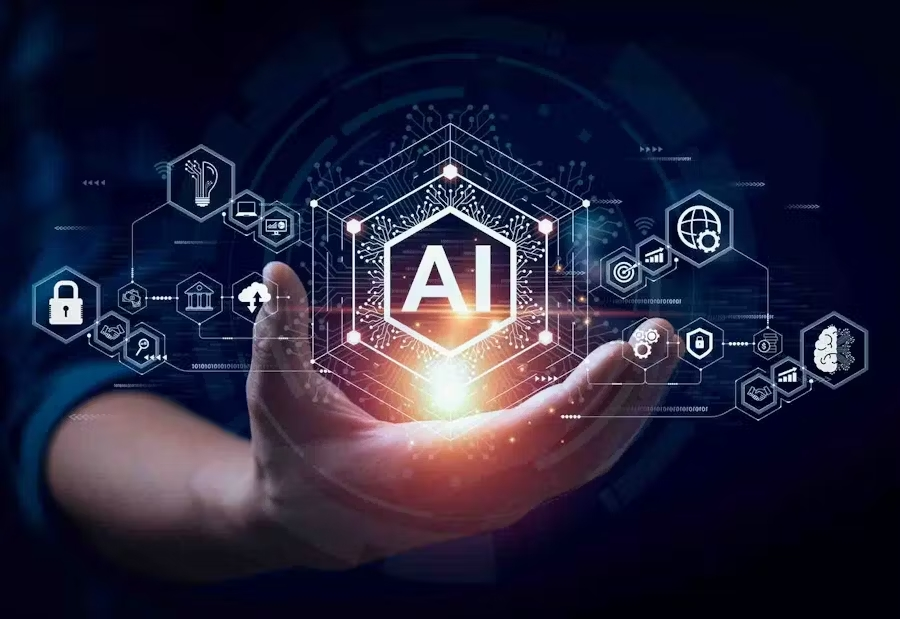
\includegraphics[width=.6\textwidth]{ramas_ia_1.jpg}
    \label{fig:my_label}
\end{figure}
    \vspace{0.2 cm}
    \begin{center}
        Inteligencia artificial y Big data \\ Córdoba, 5 de Noviembre 2024
    \end{center}
    \vspace{5 cm}
\null\hfill \textbf{Desarrollado por:}
\\
\\
\null\hfill Marta Lopez
\\
\null\hfill Víctor Páez Anguita
\clearpage
\end{titlepage}

%%%%%%%%%%%%%%%%%%%%%%%%%%%Index%%%%%%%%%%%%%%%%%%%%%%%%%%%%%%%%
\tableofcontents
\clearpage
%%%%%%%%%%%%%%%%%%%%%%%%%%%Index%%%%%%%%%%%%%%%%%%%%%%%%%%%%%%%%

\section{Introducción}

En este documento veremos los distintos usos que se le da a la Inteligencia artificial en diferentes areas
de trabajo. Además, se explicarán los beneficios que aportan a sus respectivos campos y tambíen sus desventajas.

\section{Agricultura}

\subsection{Descripción general}

La inteligencia artificial en agricultura, también conocida como AgTech, se refiere a la aplicación de tecnologías de IA para 
mejorar la eficiencia, la productividad y la sostenibilidad en la industria agrícola. Estas tecnologías permiten a los agricultores
monitorear y optimizar procesos como la siembra, el riego, la fertilización y la cosecha, mejorando la toma de decisiones y reduciendo
los costos operativos.

\subsection{Como funcionan}

\begin{itemize}
    \item Monitoreo de cultivos y análisis de suelo: 
    La IA usa imágenes satelitales y drones con sensores para monitorear cultivos y analizar el suelo.
    \item Detección de plagas y enfermedades: 
    Algoritmos de IA identifican signos tempranos de plagas y enfermedades en las plantas.
    \item Optimización del riego: 
    Sistemas de riego inteligente ajustan el agua según las necesidades de cada planta.
    \item Gestión de cosechas: 
    La IA predice los mejores momentos para la cosecha usando datos históricos y actuales.
\end{itemize}

\begin{figure}[h!]
    \centering
    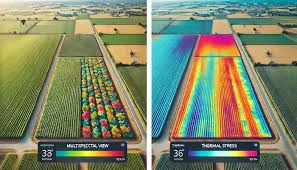
\includegraphics[width=.6\textwidth]{agricultura.png}
    \label{fig:my_label}
\end{figure}

\subsection{ventajas}

\begin{itemize}
    \item Aumento de productividad: 
    Optimiza todo el proceso agrícola, mejorando la eficiencia desde la siembra hasta la cosecha.
    \item Reducción de costos: 
    Optimiza el uso de insumos y reduce pérdidas, disminuyendo costos operativos.
    \item Sostenibilidad ambiental: 
    Favorece prácticas sostenibles al monitorear el uso de agua y aplicar insumos de forma precisa.
    \item Decisiones informadas: 
    Ofrece datos y análisis detallados, ayudando a los agricultores a tomar decisiones más acertadas.
\end{itemize}

\subsection{Desventajas}

\begin{itemize}
    \item Dependencia de la tecnología.
    \item Altos costos iniciales.
    \item Exclusión de pequeños agricultores.
\end{itemize}

\section{Banca}

\subsection{Descripción general}

La inteligencia artificial en banca se refiere a la aplicación de tecnologías de IA para mejorar la eficiencia, la seguridad y la 
experiencia del cliente en servicios financieros. Estas tecnologías permiten a los bancos automatizar procesos, detectar fraudes,
personalizar servicios y ofrecer asesoramiento financiero.

\subsection{Como funcionan}

\begin{itemize}
    \item Detección de fraudes: 
    Los algoritmos de IA identifican patrones y anomalías en grandes volúmenes de transacciones, 
    lo que permite detectar y prevenir fraudes rápidamente.
    \item Experiencias personalizadas para el cliente: 
    La IA analiza el comportamiento financiero de los clientes para ofrecer servicios personalizados, 
    y los chatbots permiten una atención al cliente eficiente las 24 horas.
    \item Automatización y eficiencia operativa: Automatiza tareas rutinarias y agiliza servicios en línea, 
    mejorando la eficiencia y reduciendo errores.
    \item Gestión de riesgos: Realiza análisis predictivos para anticipar riesgos financieros, 
    ayudando a tomar decisiones más informadas y seguras.
\end{itemize}

\begin{figure}[h!]
    \centering
    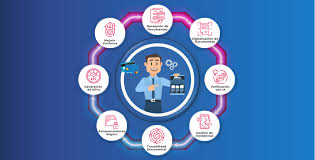
\includegraphics[width=.6\textwidth]{banca.png}
    \label{fig:my_label}
\end{figure}

\subsection{ventajas}

\begin{itemize}
    \item Mayor seguridad: 
    La IA mejora la detección de fraudes y la ciberseguridad, protegiendo a los clientes y sistemas bancarios.
    \item Eficiencia y ahorro de costes: 
    La automatización reduce costos operativos y libera recursos para tareas más complejas.
    \item Optimización de la gestión de riesgos: 
    Ofrece análisis precisos y en tiempo real para manejar riesgos y adaptarse a cambios en el mercado.
\end{itemize}

\subsection{Desventajas}

\begin{itemize}
    \item Privacidad y seguridad de datos: 
    La recopilación y análisis de datos sensibles pueden comprometer la privacidad de los clientes y requiere un cumplimiento
    riguroso de las normativas de protección de datos.
    \item Desafíos éticos: 
    Los algoritmos pueden incorporar sesgos si no se diseñan adecuadamente, lo que podría llevar a decisiones discriminatorias 
    o injustas.
    \item Dependencia tecnológica: 
    La banca depende cada vez más de los sistemas de IA, lo que puede ser un riesgo si ocurren fallos o ataques cibernéticos.    
\end{itemize}

\section{Ciberseguridad}

\subsection{Descripción general}

La inteligencia artificial en ciberseguridad se refiere a la aplicación de tecnologías de IA para proteger sistemas, redes y datos
contra amenazas cibernéticas. Estas tecnologías permiten detectar y prevenir ataques, identificar vulnerabilidades y fortalecer la
seguridad de las organizaciones.

\subsection{Como funcionan}

\begin{itemize}
    \item Detección de amenazas y anomalías: 
    La IA detecta patrones sospechosos y anomalías en tiempo real, lo que permite identificar ataques como phishing y
    malware antes de que afecten a los sistemas.
    \item Automatización de la respuesta a amenazas: 
    Automatiza la respuesta a ataques, como el aislamiento de dispositivos comprometidos, sin intervención humana.
    \item Predicción de ataques: 
    Analiza datos históricos para predecir ataques futuros y mejorar la preparación ante ciberamenazas emergentes.        
\end{itemize}

\begin{figure}[h!]
    \centering
    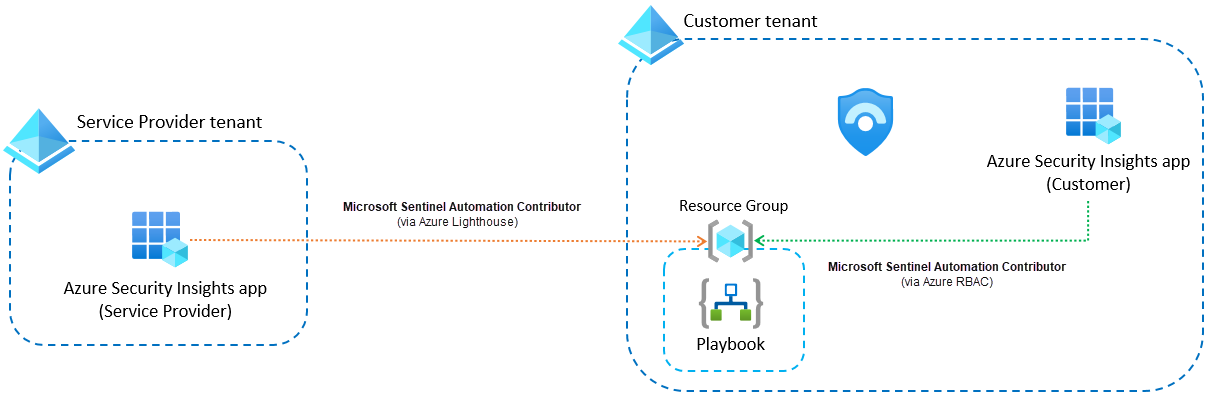
\includegraphics[width=.6\textwidth]{ciberseguridad.png}
    \label{fig:my_label}
\end{figure}

\subsection{ventajas}

\begin{itemize}
    \item Eficiencia y rapidez: 
    Detecta y neutraliza amenazas en tiempo real, minimizando daños.
    \item Reducción de la intervención humana: 
    Automatiza tareas, liberando recursos humanos para funciones más estratégicas.
    \item Prevención proactiva: 
    La IA anticipa amenazas, fortaleciendo la seguridad.
\end{itemize}

\subsection{Desventajas}

\begin{itemize}
    \item Posible uso malicioso: 
    Los ciberdelincuentes también usan IA para crear amenazas avanzadas como deepfakes y phishing más sofisticado.
    \item Riesgo de privacidad: 
    La recopilación masiva de datos personales plantea riesgos de privacidad y posibles abusos.
    \item Manipulación de modelos: 
    El envenenamiento de modelos puede alterar la efectividad de la IA y afectar la precisión en la detección de amenazas.
\end{itemize}

\section{Atención sanitaria}

\subsection{Descripción general}

La inteligencia artificial en atención sanitaria se refiere a la aplicación de tecnologías de IA para mejorar la precisión
del diagnóstico, la eficiencia en la atención al paciente y la gestión de datos médicos. Estas tecnologías permiten a los
profesionales de la salud tomar decisiones más informadas y ofrecer tratamientos personalizados.

\subsection{Como funcionan}

\begin{itemize}
    \item Análisis de datos para diagnósticos: 
    La IA ayuda a procesar rápidamente grandes volúmenes de información clínica, facilitando diagnósticos basados en
    estudios, expedientes médicos e información genética.
    \item Automatización de tareas administrativas: 
    La IA permite a los profesionales de la salud reducir el tiempo invertido en tareas rutinarias, como el manejo de
    expedientes y el ingreso de datos, liberando recursos para el cuidado directo de los pacientes.
    \item Monitoreo de salud y consultas digitales: 
    Los dispositivos y aplicaciones de monitoreo, como los relojes inteligentes, brindan datos esenciales en tiempo real. 
\end{itemize}

\begin{figure}[h!]
    \centering
    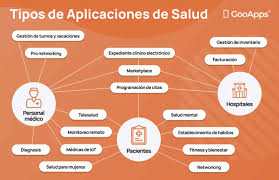
\includegraphics[width=.6\textwidth]{sanitaria.png}
    \label{fig:my_label}
\end{figure}

\subsection{ventajas}

\begin{itemize}
    \item Eficiencia y precisión: 
    La IA permite análisis detallados y rápidos, aumentando la precisión de diagnósticos y tratamientos personalizados.
    \item Reducción de carga administrativa: 
    La automatización de tareas administrativas permite que los profesionales dediquen más tiempo a la atención de los pacientes.
    \item Mayor acceso a la atención médica: 
    Con el monitoreo digital y las consultas remotas, la IA ayuda a expandir el acceso y seguimiento médico.    
\end{itemize}

\subsection{Desventajas}

\begin{itemize}
    \item Desafíos en programación y adopción: 
    Los profesionales de salud requieren capacitación en el uso de herramientas de IA, y el diseño de interfaces amigables 
    sigue siendo un desafío.
    \item Dado que la IA maneja datos sensibles: 
    Los pacientes y proveedores enfrentan riesgos y desafíos de protección de datos.
    \item Resistencia al cambio: 
    La integración de IA requiere inversiones y convencimiento sobre su efectividad, y su adopción generalizada puede ser
    lenta en un sector altamente regulado.
\end{itemize}

\section{Logística: rutas y optimización}

\subsection{Descripción general}

La inteligencia artificial en logística se refiere a la aplicación de tecnologías de IA para optimizar rutas, reducir costos y mejorar
la eficiencia en la cadena de suministro. Estas tecnologías permiten a las empresas planificar y gestionar de manera más efectiva el
transporte, el almacenamiento y la distribución de productos.

\subsection{Como funcionan}

\begin{itemize}
    \item Planificación de Rutas: 
    La IA considera variables como tráfico, clima y preferencias del cliente para crear rutas de entrega óptimas.
    \item Gestión de Inventario Inteligente: 
    Facilita el monitoreo en tiempo real de los inventarios, mejorando la toma de decisiones sobre reposición y reduciendo
    costos de almacenamiento.
    \item Automatización de Almacenes: 
    Robots impulsados por IA realizan tareas repetitivas, mejorando la eficiencia y seguridad operativa.
    \item Seguimiento en Tiempo Real: 
    Proporciona visibilidad de la cadena de suministro, ayudando a resolver problemas rápidamente.
\end{itemize}

\begin{figure}[h!]
    \centering
    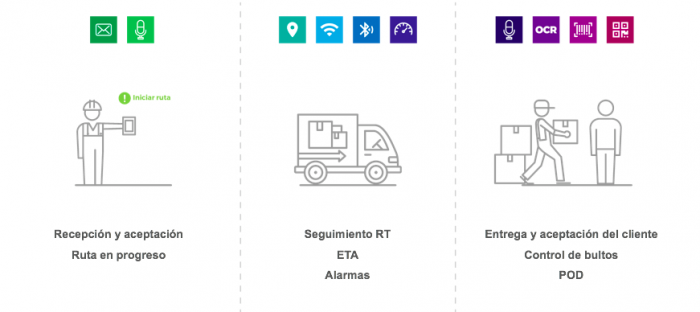
\includegraphics[width=.6\textwidth]{rutas.png}
    \label{fig:my_label}
\end{figure}

\subsection{ventajas}

\begin{itemize}
    \item Optimización de Rutas: 
    Ahorro de tiempo y costos, y reducción de la huella de carbono.
    \item Gestión de Inventario: 
    Mejor equilibrio entre oferta y demanda, aumentando la satisfacción del cliente.
    \item Automatización: 
    Robots mejoran la velocidad y precisión, reduciendo errores humanos.
    \item Mejora en la Experiencia del Cliente: 
    Información en tiempo real sobre entregas aumenta la confianza del consumidor.
    \item Análisis Predictivo: 
    Permite anticipar problemas y mejorar la eficiencia de la cadena de suministro.    
\end{itemize}

\subsection{Desventajas}

\begin{itemize}
    \item Dependencia Tecnológica: 
    Riesgo elevado en caso de fallas del sistema.
    \item Inversión Inicial Elevada: 
    Costos altos en tecnología y capacitación.
    \item Complejidad de Implementación: 
    Adaptar sistemas de IA requiere conocimientos técnicos especializados.
    \item Resistencia al Cambio: 
    La automatización puede ser mal recibida por los empleados, afectando la cultura organizacional.
\end{itemize}

\section{Telecomunicaciones: optimización de redes}

\subsection{Descripción general}

La optimización de redes en telecomunicaciones busca mejorar el rendimiento, la eficiencia y la capacidad de las redes para 
satisfacer la creciente demanda de conectividad rápida y estable. Con el aumento de dispositivos conectados y el tráfico de datos, 
es esencial optimizar las redes para evitar sobrecargas y mantener una alta calidad de servicio.

\subsection{Como funcionan}

\begin{itemize}
    \item Inteligencia Artificial (IA) y Machine Learning (ML):
    \begin{itemize}
        \item La IA y el ML permiten analizar grandes volúmenes de datos en tiempo real para optimizar el rendimiento de la red. Estas tecnologías 
        pueden predecir posibles fallos y ajustar los recursos de red en función de la demanda.
        \item Predicción de fallas: Algoritmos de ML identifican patrones que anticipan problemas en la red, lo cual permite realizar mantenimiento 
        preventivo.
        \item Automatización: La IA ajusta automáticamente parámetros de la red, como el ancho de banda, en función del tráfico actual, 
        minimizando la congestión. 
    \end{itemize}

    \item Gestión de la Calidad de Servicio (QoS):
    \begin{itemize}
        \item La QoS garantiza que aplicaciones críticas, como llamadas de voz o videoconferencias, tengan prioridad sobre aquellas menos 
        sensibles a la latencia, optimizando así la experiencia del usuario.
        \item Priorización de tráfico: Se asigna ancho de banda preferente a servicios que requieren baja latencia y se limitan aquellos de
        menor importancia en tiempo real.
        \item Control de congestión: Mediante algoritmos que monitorizan el tráfico, la red se ajusta en tiempo real para evitar sobrecargas.
    \end{itemize}


    \item Optimización del Uso del Espectro en Redes Inalámbricas:
    \begin{itemize}
        \item El espectro es un recurso limitado en telecomunicaciones, y optimizar su uso es esencial para maximizar la capacidad de la red 
        sin afectar la calidad de la conexión.
        \item MIMO (Multiple Input Multiple Output): Aprovecha múltiples antenas para reducir la interferencia y mejorar la capacidad de la red.
        \item Celdas pequeñas y femtoceldas: Estas soluciones ayudan a cubrir áreas de alta demanda mediante el uso de celdas de menor alcance, 
        lo que reduce la carga en la red principal y mejora la cobertura.
        \item Agrupamiento de portadoras: Utilizado en tecnologías 4G y 5G, combina diferentes bandas de frecuencia para mejorar la velocidad 
        y estabilidad de la conexión.
    \end{itemize}

    \item Optimización de Redes de Acceso y Núcleo:
    \begin{itemize}
        \item Las redes de acceso y núcleo (core) conectan dispositivos con la infraestructura central de la red y son fundamentales para la 
        eficiencia y confiabilidad general.
        \item Redes Definidas por Software (SDN): Permiten una gestión centralizada de los flujos de datos mediante software, lo cual 
        optimiza el uso de recursos y permite configuraciones flexibles.
        \item Virtualización de Funciones de Red (NFV): Reemplaza equipos físicos por software, lo cual reduce costos y permite escalar 
        los recursos de manera más eficiente.
    \end{itemize}

\end{itemize}

\begin{figure}[h!]
    \centering
    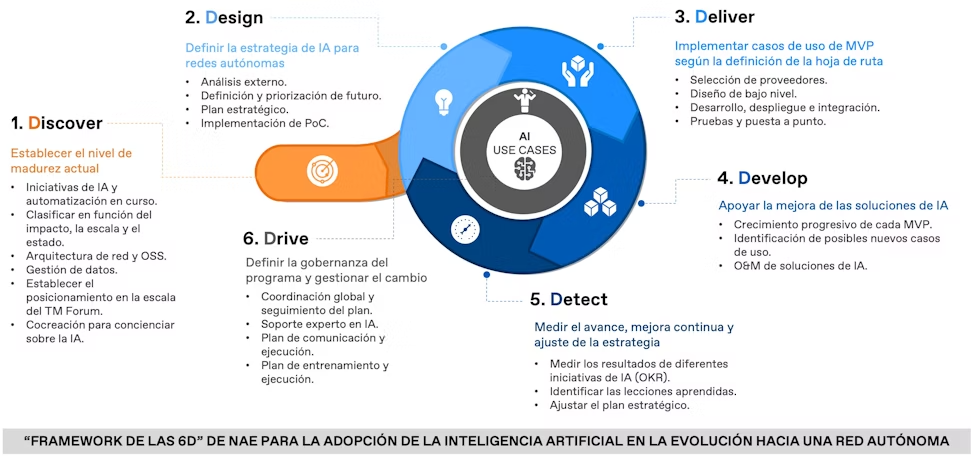
\includegraphics[width=.6\textwidth]{teleco.png}
    \label{fig:my_label}
\end{figure}

\subsection{ventajas}
\begin{itemize}
    \item Mejora en la calidad del servicio: 
    Reduce la latencia y mejora la estabilidad en servicios como videollamadas y juegos en línea.
    \item Uso eficiente de recursos: 
    Optimiza el uso del espectro y reduce los costos operativos mediante la virtualización y el SDN.
    \item Mantenimiento predictivo: 
    Evita fallas en la red, minimizando el tiempo de inactividad y aumentando la disponibilidad.
\end{itemize}

\subsection{Desventajas}
\begin{itemize}
    \item Costos de implementación: 
    Integrar IA, ML y virtualización requiere una inversión inicial significativa.
    \item Dependencia de la tecnología: 
    La automatización y el control centralizado pueden ser vulnerables a fallos en los sistemas de software.
    \item Riesgos de seguridad: 
    La optimización y virtualización aumentan los puntos de vulnerabilidad en la red, lo cual exige medidas de ciberseguridad adicionales.
\end{itemize}

\section{Juegos: creación de agentes inteligentes}

\subsection{Descripción general}
Los agentes inteligentes en videojuegos son sistemas de IA diseñados para simular el comportamiento humano o para actuar de manera
autónoma en función de un entorno o de las acciones del jugador. Estos agentes mejoran la jugabilidad y la experiencia al reaccionar 
de manera dinámica e imitar la toma de decisiones humanas.
\subsection{Como funcionan}
\begin{itemize}
    \item Modelos basados en reglas:
    Este es el enfoque más sencillo, donde los personajes o agentes actúan según un conjunto de reglas preestablecidas. 
    Estos modelos tienen limitaciones, ya que no se adaptan a nuevas situaciones.
    \item Aprendizaje por refuerzo: 
    Utilizado especialmente en juegos que requieren agentes adaptativos. 
    En este enfoque, el agente toma decisiones basadas en recompensas o penalizaciones, mejorando su comportamiento a 
    medida que aprende cuáles acciones son óptimas. Un ejemplo de esto es AlphaGo, que aprendió a jugar al juego de mesa Go, 
    superando a jugadores humanos.
    \item Redes neuronales y algoritmos evolutivos: 
    Permiten que el agente aprenda de patrones complejos y ajuste su comportamiento en tiempo real, incluso sin reglas explícitas, 
    solo observando el entorno. Los algoritmos evolutivos pueden “cruzar” las características de los agentes exitosos, permitiendo a 
    los agentes evolucionar con el tiempo.
\end{itemize}

\begin{figure}[h!]
    \centering
    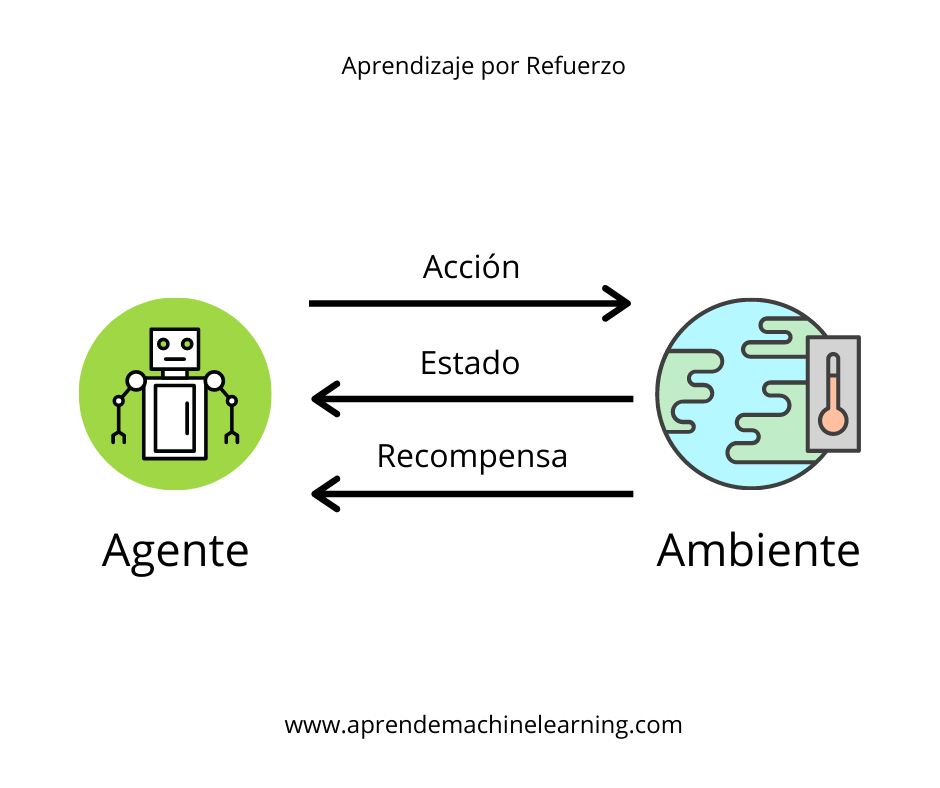
\includegraphics[width=.5\textwidth]{AprendizajeRefuerzo-global.png}
    \label{fig:my_label}
\end{figure}

\clearpage

\subsection{ventajas}
\begin{itemize}
    \item Los agentes pueden crear experiencias de juego desafiantes y adaptativas.
    \item Los jugadores pueden enfrentarse a oponentes de IA que evolucionan y se vuelven más sofisticados.
\end{itemize}

\subsection{Desventajas}
\begin{itemize}
    \item El comportamiento de la IA puede volverse impredecible o incluso frustrante si es demasiado difícil.
    \item El desarrollo y la optimización de agentes inteligentes requieren muchos recursos.
\end{itemize}

\section{Arte: Creatividad}
\subsection{Descripción general}

La inteligencia artificial en arte implica la generación de imágenes, estilos y composiciones visuales. Estas creaciones suelen 
combinarse con el trabajo humano o se generan por completo mediante IA, resultando en obras de arte que, en algunos casos, no son 
distinguibles de las creadas por humanos.

\subsection{Como funcionan}
\begin{itemize}
    \item Redes Generativas Antagónicas (GAN): 
    Las GAN constan de dos redes neuronales (generador y discriminador) que compiten entre sí. El generador intenta crear imágenes 
    convincentes mientras que el discriminador evalúa si son reales o artificiales, perfeccionando así la calidad de las imágenes generadas. 
    Este tipo de red es ideal para crear obras de arte nuevas y únicas.
    \item Transferencia de estilo neuronal: 
    En este proceso, un modelo de IA aplica el estilo de una obra de arte a otra imagen. 
    Esto se logra extrayendo y combinando patrones de color y forma, permitiendo que una fotografía, 
    por ejemplo, se asemeje al estilo de Van Gogh o Picasso.

\clearpage

    \item Procesamiento de imágenes:
    Modelos de visión artificial detectan patrones y crean nuevas composiciones basadas en elementos artísticos conocidos. 
    También permiten realizar modificaciones como ajustes de color y estilo, basándose en grandes bases de datos de imágenes.
\end{itemize}

\begin{figure}[h!]
    \centering
    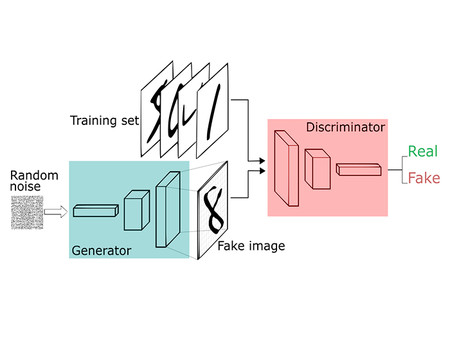
\includegraphics[width=.6\textwidth]{GAN.jpg}
    \label{fig:my_label}
\end{figure}


\subsection{ventajas}
\begin{itemize}
    \item Democratiza la creación de arte y permite a cualquier persona experimentar con el arte digital.
    \item Amplía las posibilidades creativas, ofreciendo nuevas formas de expresión artística y herramientas colaborativas.
\end{itemize}

\subsection{Desventajas}
\begin{itemize}
    \item Puede llevar a la desvalorización del trabajo artístico humano y a una posible dependencia de la IA para la creatividad.
    \item La IA podría imitar estilos sin consentimiento, generando riesgos de apropiación cultural.
\end{itemize}

\section{Escritura: corrección y generación de texto}

\subsection{Descripción general}
La IA en el ámbito de la escritura facilita la corrección automática, la generación de texto y la asistencia en redacción. 
Estos modelos permiten a los usuarios escribir con menos errores gramaticales, mejorar el estilo y generar contenido automáticamente 
en diferentes contextos.

\subsection{Como funcionan}
\begin{itemize}
    \item Modelos de lenguaje: 
    Los modelos de lenguaje actuales como GPT (Generative Pre-trained Transformer), BERT (Bidirectional Encoder Representations from Transformers)
    y T5 (Text-To-Text Transfer Transformer) se entrenan con grandes volúmenes de texto para predecir las palabras siguientes en una oración. 
    Estos modelos pueden generar texto coherente que se ajusta al contexto dado.
    \item Corrección gramatical:
    Utilizan modelos supervisados que identifican errores en el texto basándose en patrones de contexto. Estas herramientas son especialmente 
    útiles en software de edición de texto como Grammarly.
    \item Generación creativa de texto:
    Las IA como ChatGPT generan contenidos narrativos, académicos o incluso publicitarios, ajustándose al tono, estilo y longitud deseados.
\end{itemize}

\begin{figure}[h!]
    \centering
    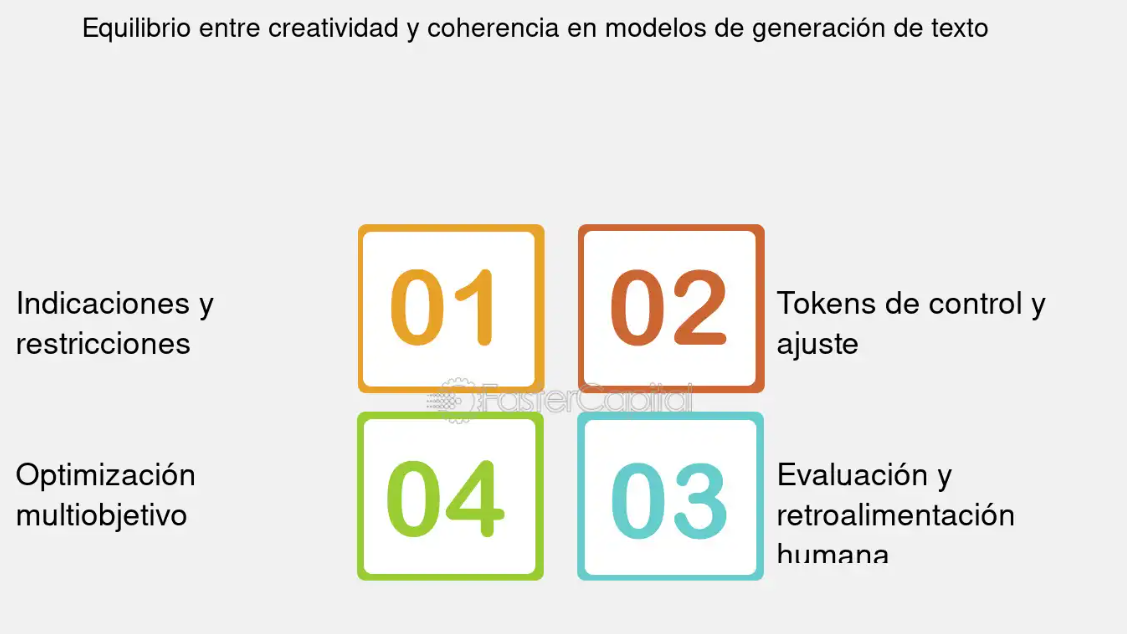
\includegraphics[width=.6\textwidth]{generacionCreativa.PNG}
    \label{fig:my_label}
\end{figure}

\subsection{ventajas}
\begin{itemize}
    \item Mejora la accesibilidad y facilita la redacción sin errores gramaticales.
    \item Puede ahorrar tiempo en la creación de contenido, desde artículos informativos hasta literatura creativa.
\end{itemize}

\subsection{Desventajas}
\begin{itemize}
    \item Existe el riesgo de creación de contenido repetitivo o con sesgo.
    \item Plantea preocupaciones éticas sobre la autoría y el plagio en la generación de textos automatizados.
\end{itemize}

\clearpage

\section{Conclusiones}

La inteligencia artificial ha transformado numerosos campos, desde la agricultura y la banca hasta la atención sanitaria y 
la logística. Los beneficios de la IA incluyen una mayor eficiencia, una toma de decisiones más informada y una mayor
personalización de servicios. Sin embargo, también plantea desafíos como la dependencia tecnológica, la privacidad de los datos
y la resistencia al cambio. A medida que la IA continúa evolucionando, es esencial abordar estos desafíos y maximizar los beneficios
que esta tecnología puede aportar a la sociedad.
Sin embargo la IA no solo se limita a estos campos, sino que también se ha expandido a otros como la creación de arte, la escritura
y los videojuegos, demostrando su versatilidad y su capacidad para innovar en diferentes áreas. A medida que la IA continúa evolucionando,
es fundamental abordar los desafíos éticos, legales y de seguridad que plantea, garantizando que se utilice de manera responsable y
beneficiosa para la sociedad.

\clearpage

\section{Bibliografia}
\begin{itemize}
    \item \href{https://www.cafi.org.ar/como-se-aplica-la-ia-en-la-agricultura-y-algunos-ejemplos/}{CAFI}
    \item \href{https://vasscompany.com/es/insights/blogs-articles/ia-en-banca-beneficios-y-riesgos/}{VASS}
    \item \href{https://blog.outvise.com/impacto-de-inteligencia-artificial-en-ciberseguridad/}{OUTVISE}
    \item \href{https://driv.in/blog/beneficios-de-ia-logistica}{DRIV.IN}
    \item \href{https://www.redhat.com/es/topics/hyperconverged-infrastructure/what-is-software-defined-networking}{RedHat}.
    \item \href{https://r9.ieee.org/ecuador-magaz/rendimiento-y-modelamiento-de-sistemas-de-comunicacion-inalambrica-5g%E2%80%8B/}{MagazIEEE}.
    \item \href{https://www.iic.uam.es/innovacion/alphazero-y-el-go/}{Instituto de ingeniería del conocimiento}.
    \item \href{https://theblackboxlab.com/2024/02/23/deepmind/}{The blackBoxLab}.
    \item \href{https://www.linkedin.com/pulse/creatividad-artificial-est%C3%A1-la-ia-redefiniendo-el-concepto-e0djc/}{Sube Consultores}.
    \item \href{https://www.technologyreview.es/s/16532/que-es-la-inteligencia-artificial}{MIT technology review}.
    \item \href{https://www.sciencedirect.com/science/article/pii/S1136103423000114}{ScienceDirect}.
    \item \href{chrome-extension://efaidnbmnnnibpcajpcglclefindmkaj/https://www.reue.org/wp-content/uploads/2024/07/184-195.pdf}{REUE | Artículo especial}.


\end{itemize}

\end{document}
